\documentclass[user_manual.tex]{subfiles}
\begin{document}
\chapter{Puesta en marcha}
En este capitulo se explicara de forma concisa el uso y funcionamiento del robot de forma practica, así como mostrar alternativas para el uso de los nodos sin contar con el hardware del robot. Como primera instancia se ilustrara la forma de conexión entre las dos computadoras (las cuales fueron mencionadas en el capitulo 3 primeros pasos), así como la conexión de esta con el hardware de Justina.

\section{Conexión ubuntu-plateada}
Conexión

\section{RViz}
Para probar el funcionamiento del hardware y software de Justina se puede utilizar RViz y la GUI. Para ejecutar estos programas se puede hacer uso de diferentes launche y run de ros.

\section{GUI}
GUI
\section{Pruebas}
\begin{minted}[
frame=lines,
framesep=1mm,
bgcolor=black,
baselinestretch=1.2
]{console}
 ~$ roslaunch surge_et_ambula justina.launch
\end{minted}
%$

 \begin{center}
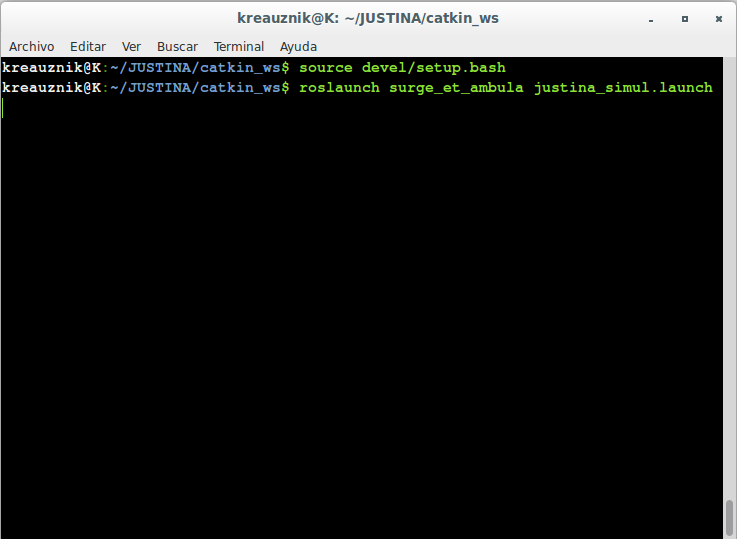
\includegraphics[width=0.73\textwidth]{Figures/PP/pp6.png}
\end{center}
\section{Simulación en el RViz y GUI de Justina}
Una alternativa para utilizar el software y hacer pruebas cuando no se cuenta con el hardware es utilizar la simulación de Rrviz y GUI, para esto se debe ejecutar el siguiente comando:\\
\\
\begin{minted}[
frame=lines,
framesep=1mm,
bgcolor=black,
baselinestretch=1.2
]{console}
 ~$ roslaunch surge_et_ambula justina_simul.launch
\end{minted}
%$\\
\\
Esto nos permite ocupar funciones del software de Justina, pero no es posible ocupar todas ya que algunas son dependientes de hardware y este es necesario para su correcto funcionamiento. Está opción para ocupar Rviz y GUI puede ocupar muchos recursos por lo que a continuación se dispodran algunas pruebas que pueden ser ejecutadas sin necesidad del hardware.


\end{document}